\documentclass[unknownkeysallowed]{beamer}
\mode<presentation>
{
%  \usetheme{AnnArbor}
%  \usetheme{Dresden}
%  \usetheme{Montpellier}
%  \usetheme{Antibes}
%  \usetheme{Frankfurt}
%  \usetheme{PaloAlto}
%  \usetheme{Bergen}
%  \usetheme{Boadilla}
%  \usetheme{Goettingen}
%  \usetheme{Pittsburgh}	%!!
%  \usetheme{Berkeley}
%  \usetheme{Hannover}
%  \usetheme{Rochester}		%!!!
%  \usetheme{Berlin}
%  \usetheme{Ilmenau}
%  \usetheme{Singapore}
  \usetheme{Boadilla}		%viel platz
%  \usetheme{JuanLesPins}
%  \usetheme{Szeged}		%!
%  \usetheme{boxes}
%  \usetheme{Luebeck}
%  \usetheme{Warsaw}
%  \usetheme{Copenhagen}
%  \usetheme{Madrid}
%  \usetheme{Darmstadt}
%  \usetheme{Malmoe}
%  \usetheme{default}
%  \usetheme{JuanLesPins}

%  \usetheme{Marburg}


%\usefonttheme{professionalfonts}
%	default | professionalfonts | serif |
%	structurebold | structureitalicserif |
%	structuresmallcapsserif
%\useinnertheme{rounded}
%	circles | default | inmargin |
%	rectangles | rounded

%  \setbeamercovered{transparent}
  % oder auch nicht
\usecolortheme{rose}


\definecolor{uaf yellow}{cmyk}{0,0.16,1,0} % official UAF yellow
\definecolor{light yellow}{cmyk}{0.01,0,0.16,0}
\definecolor{uaf blue}{cmyk}{1,0.66,0,0.02} % official UAF blue
\definecolor{light blue}{cmyk}{0.22,0.11,0,0}
\definecolor{arsc blue}{HTML}{005496}
\definecolor{arsc red}{HTML}{a20a42}
\definecolor{arsc green}{HTML}{009a82}
\definecolor{light gray}{HTML}{777777}

  %navigation aus, klaut nur platz
  \setbeamertemplate{navigation symbols}{}
% Reset title background to default
%\setbeamertemplate{title page}[default]
\setbeamercolor{title}{bg=}
\setbeamercolor{frametitle}{bg=uaf blue, fg=white}
\setbeamercolor{institute}{fg=white}
\setbeamercolor{date}{fg=white}
\setbeamercolor{block}{bg=}
%\setbeamercolor{title}{fg=black}

% Reset block background to default
%\setbeamertemplate{blocks}[default]
%\setbeamercolor{block title}{bg=}
%\setbeamercolor{block body}{bg=}

\beamertemplatenavigationsymbolsempty  
\setbeamertemplate{blocks}[rounded][shadows=false]

\useinnertheme{circles}

}
\usepackage[latin1]{inputenc}
\usepackage{latexsym}
\usepackage{amsfonts}
%\usepackage{natbib}
\usepackage{fancyhdr}
\usepackage{graphicx}
%\usepackage{subfigure}
% oder was auch immer
\usepackage{grffile}
\usepackage{pgf}
\usepackage{tikz}

\usepackage{listings}

\usepackage{times}
\usepackage[T1]{fontenc}
%\usepackage{appendixnumber}
% Oder was auch immer. Zu beachten ist, das Font und Encoding passen
% müssen. Falls T1 nicht funktioniert, kann man versuchen, die Zeile
% mit fontenc zu löschen.

\hypersetup{
    bookmarks=true,         % show bookmarks bar?
    unicode=false,          % non-Latin characters in Acrobat's bookmarks
    pdftoolbar=true,        % show Acrobat's toolbar?
    pdfmenubar=true,        % show Acrobat's menu?
    pdffitwindow=false,     % window fit to page when opened
    pdfstartview={FitH},    % fits the width of the page to the window
    pdftitle={My title},    % title
    pdfauthor={Author},     % author
    pdfsubject={Subject},   % subject of the document
    pdfcreator={Creator},   % creator of the document
    pdfproducer={Producer}, % producer of the document
    pdfkeywords={keyword1} {key2} {key3}, % list of keywords
    pdfnewwindow=true,      % links in new window
    colorlinks=false,       % false: boxed links; true: colored links
    linkcolor=red,          % color of internal links
    citecolor=green,        % color of links to bibliography
    filecolor=magenta,      % color of file links
    urlcolor=cyan           % color of external links
}

\title[PAG]% (optional, nur bei langen Titeln nötig)
{GEOS 436 / 636\\
Programming and Automation for Geoscientists\\[20pt]
-- Week 12: Generic Mapping Tools via pyGMT --
}

\author[Grapenthin]% (optional, nur bei vielen Autoren)
{Ronni Grapenthin\\
rgrapenthin@alaska.edu\\
Elvey 413B\\
x7682}
% - Namen müssen in derselben Reihenfolge wie im Papier erscheinen.
% - Der \inst{?} Befehl sollte nur verwendet werden, wenn die Autoren
%   unterschiedlichen Instituten angehören.

\institute[UAF] % (optional, aber oft nötig)
{}
% - Der \inst{?} Befehl sollte nur verwendet werden, wenn die Autoren
%   unterschiedlichen Instituten angehören.
% - Keep it simple, niemand interessiert sich für die genau Adresse.

% - Namen müssen in derselben Reihenfolge wie im Papier erscheinen.
% - Der \inst{?} Befehl sollte nur verwendet werden, wenn die Autoren
%   unterschiedlichen Instituten angehören.

% - Der \inst{?} Befehl sollte nur verwendet werden, wenn die Autoren
%   unterschiedlichen Instituten angehören.
% - Keep it simple, niemand interessiert sich für die genau Adresse.

\date[]{}

% - Volle oder abgekürzter Name sind möglich.
% - Dieser Eintrag ist nicht für das Publikum gedacht (das weiß
%   nämlich, bei welcher Konferenz es ist), sondern für Leute, die diese
%   Folien später lesen.

%\AtBeginSection[]
%{
%  \begin{frame}<beamer>
%    \frametitle{Outline}
%    \tableofcontents[currentsection,currentsubsection]
%  \end{frame}
%}

% Falls Aufzählungen immer schrittweise gezeigt werden sollen, kann
% folgendes Kommando benutzt werden:

%\beamerdefaultoverlayspecification{<+->}

%%switch on to have only frame numbers
\setbeamertemplate{footline}[frame number]

\defbeamertemplate*{title page}{customized}[1][]
{
		\begin{tikzpicture}
			\node[text width=\textwidth,
				fill=gray!70, 
				fill opacity=0.75,
				text opacity=1,
				rounded corners = 10pt,
				inner sep=2pt]{
				\begin{center}	
			  \usebeamerfont{title}{\bf \usebeamercolor[fg]{title} \inserttitle}
			  \par
			  \usebeamerfont{subtitle}\insertsubtitle\par
			  \bigskip
			  \usebeamerfont{author}\insertauthor\par
			  \bigskip
			  \usebeamerfont{institute}\insertinstitute\par
			  \bigskip
			  \usebeamerfont{date}\insertdate\par
			  \end{center}
			  };
	\end{tikzpicture}		  
%	\vspace{0.4cm}\usebeamercolor[fg]{titlegraphic}\inserttitlegraphic 
%	\begin{flushright}
%	\vspace{-1.25cm}\includegraphics[width=2cm]{../moore_logo_transp.png}\vspace{5cm}
%	\end{flushright}
}

\begin{document}

\lstset{numbers=left, numberstyle=\tiny, stepnumber=2, basicstyle=\ttfamily, numbersep=5pt, xleftmargin=10pt}

\setbeamertemplate{background}{\includegraphics[width=\paperwidth]{/home/roon/Pictures/rooftop_initial.jpg}}

	\begin{frame}
	\begin{center}
		\titlepage
	\end{center}
	\end{frame}

\setbeamertemplate{background}{}

\begin{frame}
\frametitle{}
%	\vspace{2cm}
	How to automate making publication-quality:

	\begin{itemize}
		\item maps,
		\item x-y plots, 
		\item animations 
	\end{itemize}

	using world class base data sets while having maximum flexibility regarding layout of your product?
\end{frame}


\begin{frame}
\frametitle{}
	\begin{center}
		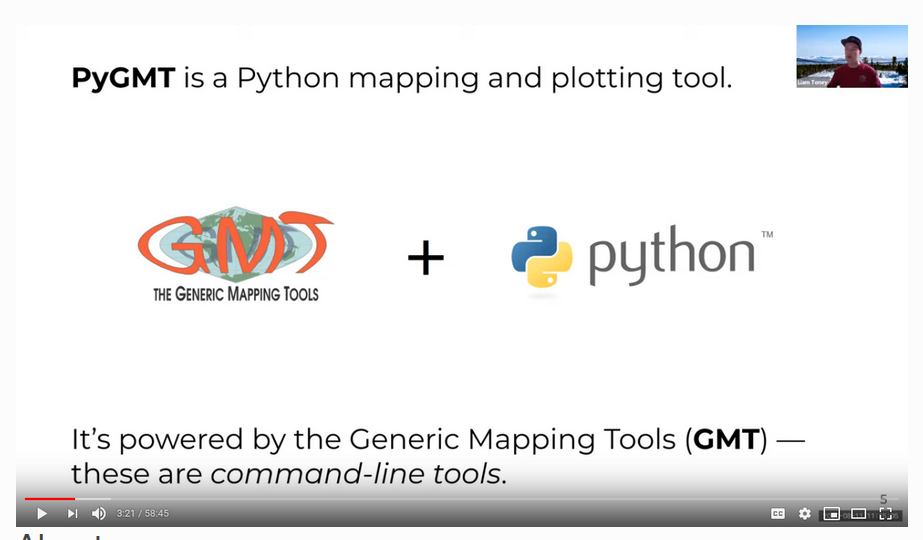
\includegraphics[width=\textwidth]{../figures/pygmt_header.png}	
	\end{center}
	\begin{flushright}
	\tiny{\emph{\url{https://www.pygmt.org/latest/index.html}}}
	\end{flushright}	
\end{frame}

\begin{frame}
\frametitle{pyGMT Goals}
	\vspace{-0.25cm}
	\begin{center}
		
\includegraphics[width=\textwidth]{../figures/pygmt_goals.png}
	\end{center}
	\begin{flushright}
	\vspace{-0.15cm}
	\tiny{\emph{\url{https://www.pygmt.org/latest/index.html}}}
	\end{flushright}	
\end{frame}

\begin{frame}[fragile=singleslide]
\frametitle{pyGMT.Figure - base class}
	\begin{center}
			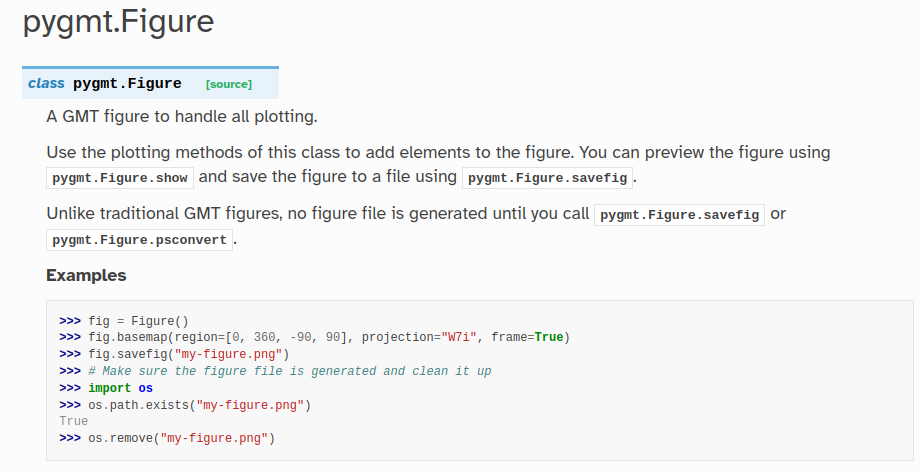
\includegraphics[width=\textwidth]{../figures/pygmt_figure.png}	
	\end{center}
	\begin{flushright}
	\vspace{-0.35cm}
	\tiny{\emph{\url{https://www.pygmt.org/latest/api/generated/pygmt.Figure.html\#pygmt.Figure}}}
	\end{flushright}	
\end{frame}

\begin{frame}[fragile=singleslide]
\frametitle{pyGMT.Figure - methods}
	\begin{center}
			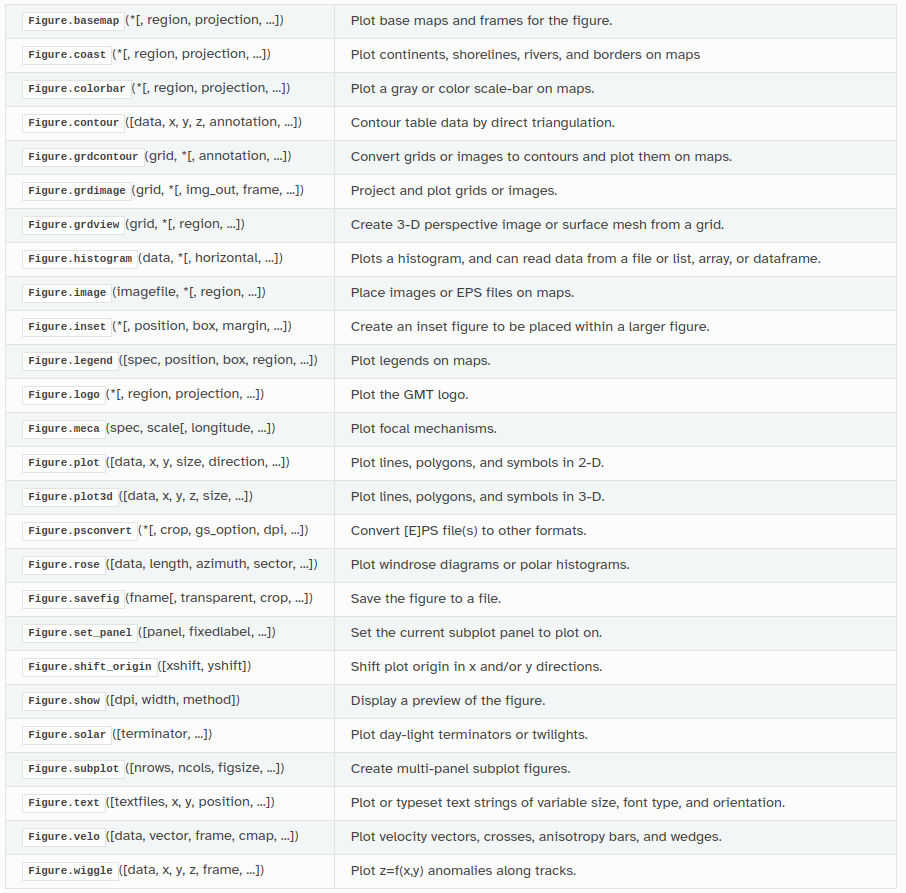
\includegraphics[width=\textwidth]{../figures/pygmt_figure_methods.png}	
	\end{center}
	\begin{flushright}
	\vspace{-0.35cm}
	\tiny{\emph{\url{https://www.pygmt.org/latest/api/generated/pygmt.Figure.html\#pygmt.Figure}}}
	\end{flushright}	
\end{frame}


\begin{frame}[fragile=singleslide]
\frametitle{pyGMT comes loaded - Datasets}
	\begin{center}
			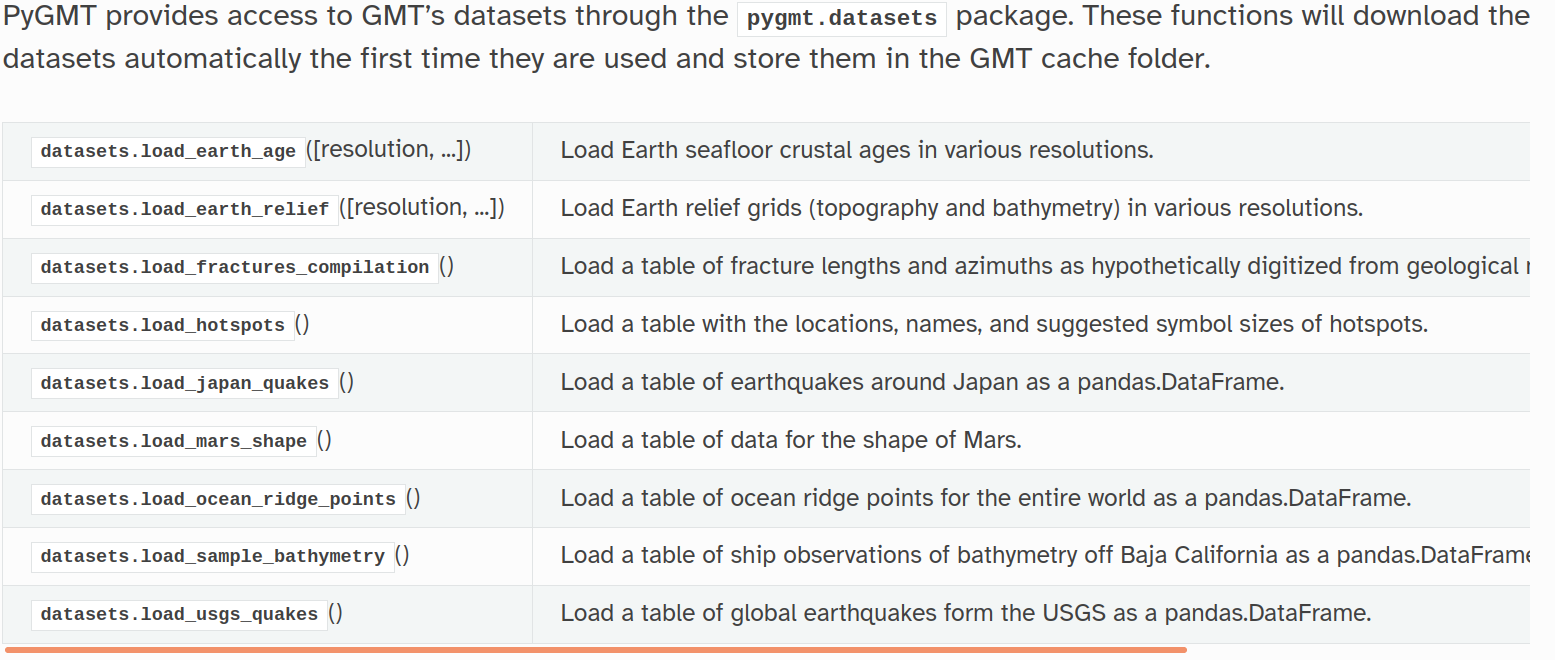
\includegraphics[width=\textwidth]{../figures/pygmt_datasets.png}	
	\end{center}
	\begin{flushright}
	\vspace{-0.35cm}
	\tiny{\emph{\url{https://www.pygmt.org/latest/api/index.html\#datasets}}}
	\end{flushright}	
\end{frame}


\begin{frame}
\frametitle{pyGMT comes loaded - Coastlines}
	\begin{center}
			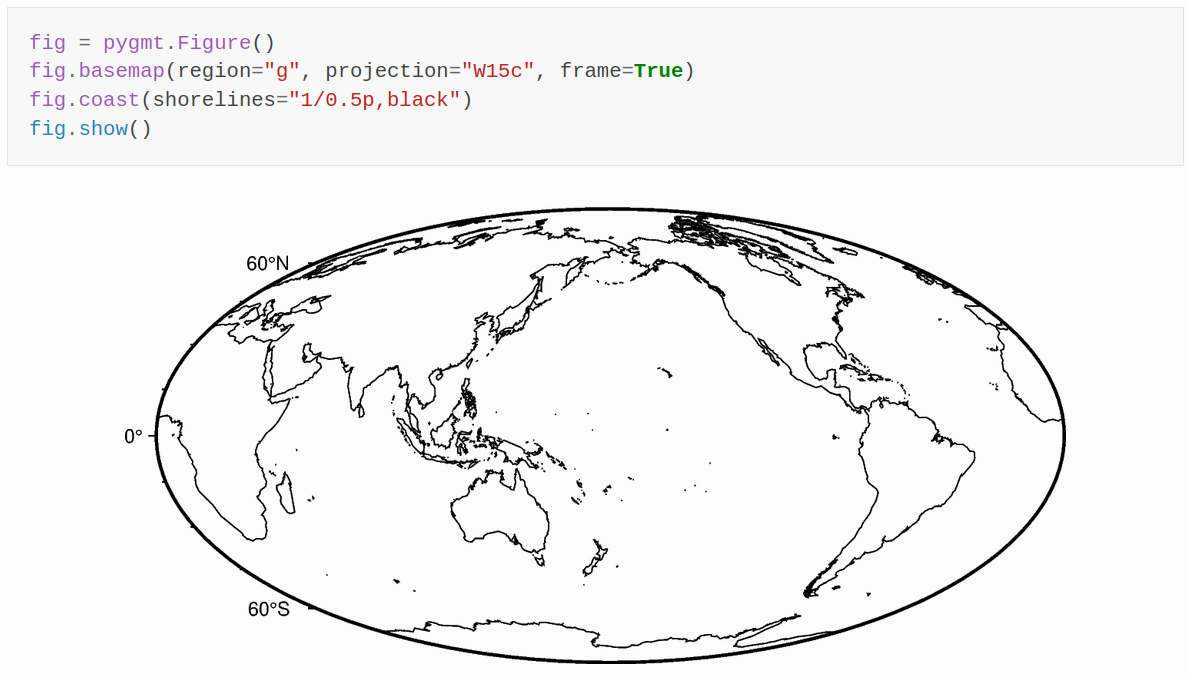
\includegraphics[width=\textwidth]{../figures/pygmt_coastlines.png}	
	\end{center}
	\begin{flushright}
	\vspace{-0.35cm}
	\tiny{\emph{\url{https://www.pygmt.org/latest/tutorials/coastlines.html}}}
	\end{flushright}	

\end{frame}

\begin{frame}[fragile=singleslide]
\frametitle{GMT comes loaded - The 31 Projections}
	\begin{center}
			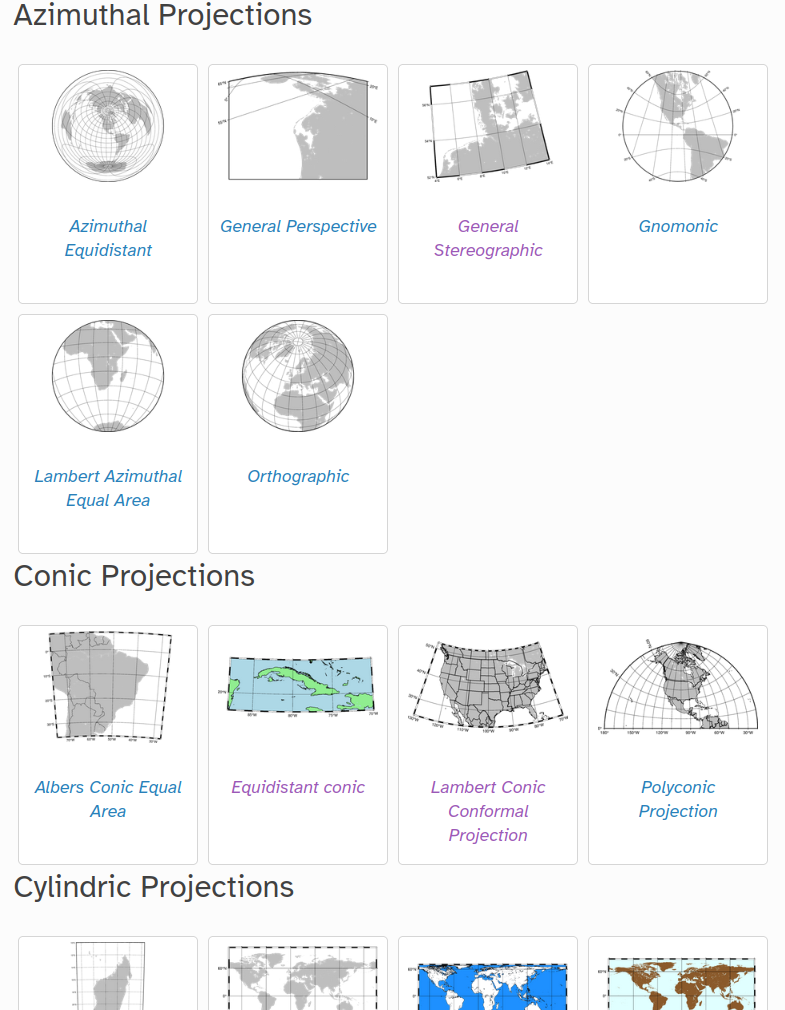
\includegraphics[width=.75\textwidth]{../figures/pygmt_projections.png}	
	\end{center}
	\begin{flushright}
	\vspace{-0.35cm}
	\tiny{\emph{\url{https://www.pygmt.org/latest/projections/index.html}}}
	\end{flushright}	

\end{frame}

\begin{frame}[fragile=singleslide]
\frametitle{GMT comes loaded - The 31 Projections}
	\begin{center}
			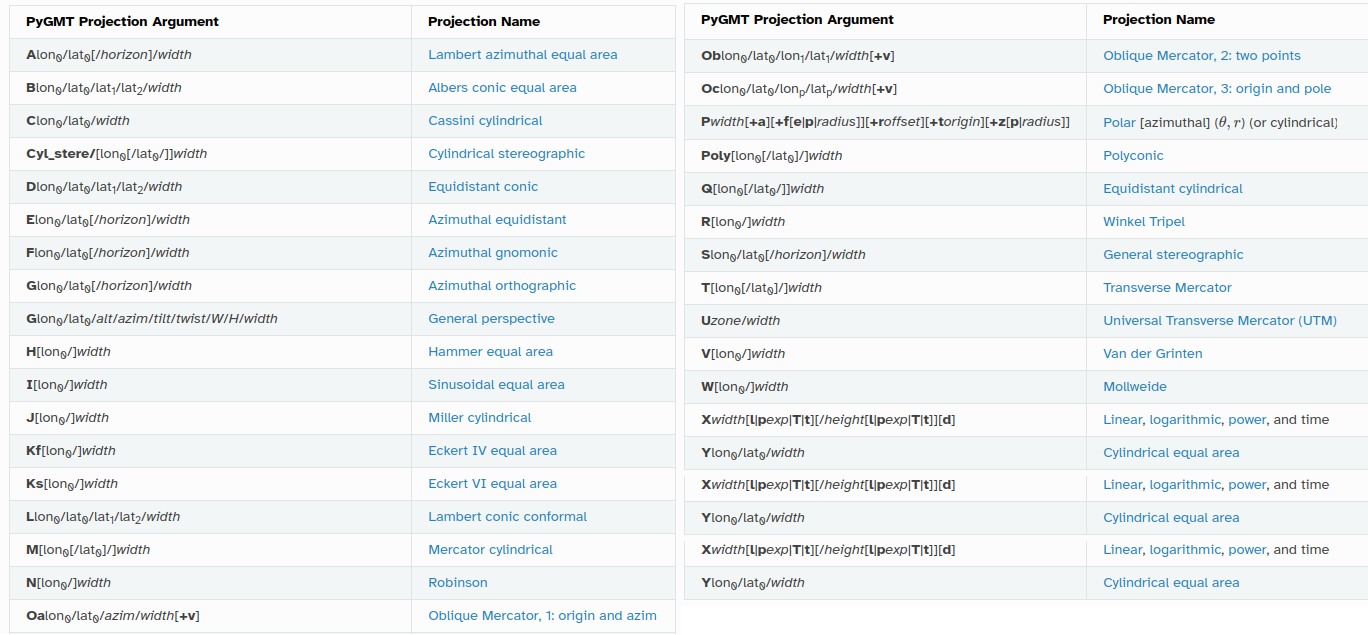
\includegraphics[width=\textwidth]{../figures/pygmt_projections_list.png}	
	\end{center}
	\begin{flushright}
	\vspace{-0.35cm}
	\tiny{\emph{\url{https://www.pygmt.org/latest/projections/index.html}}}
	\end{flushright}	

\end{frame}


\end{document}
